\section{Analiza danych}
Ogólna tendencja - im większy rozmiar pakietu oraz krótszy odstęp, tym  szybsze tempo wyłączania się węzłów sieci.

Algorytmy Flood oraz SPIN wykazują jednakowe tempo spadku liczby aktywnych czujników, niezależne od rozmiaru pakietu oraz okresu między pakietami. W przypadku również większość czujników wyłącza się w bardzo krótkim przedziale czasowym. Oznacza to, że zużycie energii przez węzły jest równomierne (wszystkie czujniki są przez cały czas swojej aktywności w trybie nasłuchiwania - w przeciwieństwie do rodziny alogrytmów typu LEACH, w których występują okresy ''uśpienia'' czujników).

Sieci korzystające z protokołów LEACH, ALEACH i LEACH DCHS wykazują wyraźnie dłuższe działanie niż sieci używające Flood i SPIN.
Różnice zacierają się dla większych rozmiarów pakietów i mniejszych odstępów czasu pomiędzy pakietami.

Różnice pomiędzy grupami protokołów są wyraźniejsze dla sieci z liczbą węzłów 200.

Poniższe wykresy przedstawiają liczbę aktywnych węzłów sieci w czasie oraz w zależności od rozmiaru pakietu i odstępie czasu pomiędzy kolejnymi pakietami. Sieć składała się z dwudziestu węzłów, które rozmieszczone zostały zgodnie z rozkładem normalnym.
Przy rozmiarach pakietu wynoszących 50B i 500B najdłuższy czas działania sieci osiągnięto wykorzystując protokół ALEACH. Czas działania sieci używających wariantów protokołu LEACH uległ wyraźnemu skróceniu przy rozmiarze pakietu wynoszącym 5000B. Wpływ okres pomiędzy pakietami na protokoły typu LEACH jest również zauważalny, jednakże jest on zdecydowanie mniej wyrazisty. Czas działania sieci dla protokołów Flood i SPIN pozostaje niezmienny, niezależnie od dobranych parametów wykresu. Dodatkowo w ich przypadku deaktywacja węzłów sieci przebiega gwałtownie oraz lawinowo - większość węzłów sieci zostaje wyłączonych w okolicach jednego punktu w czasie.

Przy rozmiarze pakietu 5B najlepszymi protokołami z punktu widzenia całkowitej długości życia sieci okazały się ALEACH oraz LEACH DCHS.

Przy rozmiarze pakietu 50B najlepszym protokołem z punktu widzenia całkowitej długości życia sieci okazał się ALEACH. W przypadku okresu między pakietami wynoszącym 20s zapewnił on około 50s dłuży czas działania sieci, jednakże protokoły LEACH oraz LEACH DCHS zapewniły dłuży okres jej stabilnego działania.

Przy rozmiarze pakietu 500B wśród protokołów umożliwiających najdłuższe działanie sieci znajduje się ALEACH. Przy okresie 10s LEACH działa lepiej od LEACH DCSH, a w przy okresie 5s i 20s LEACH DCSH działa dłużej niż LEACH.

\clearpage
\thispagestyle{empty}

 {\pdfpagewidth=2\pdfpagewidth
    \vspace*{-2cm}
    \noindent\kern.5\pdfpagewidth\rlap{\parbox{\textwidth}{%
    \noindent\kern.25\pdfpagewidth
        \llap{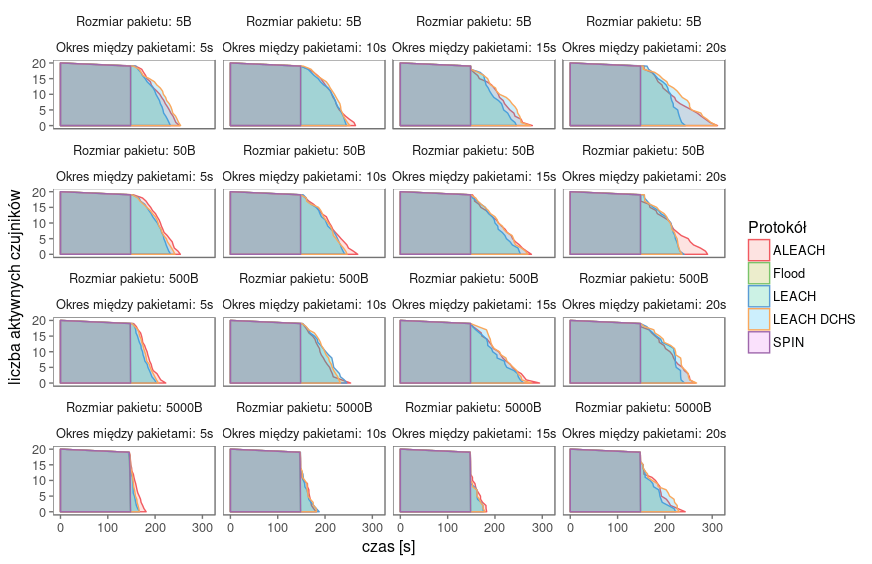
\includegraphics[width=308mm,height=229mm,page=1]{\ImgPath/charts/alive_nodes_normal_20sensors.png}}\endgraf
    \vspace{2ex}%
    \captionof{figure}{Aktywne węzły - 20 czujników, rozkład normalny}}}\kern-.5\pdfpagewidth
     \par
     \vspace*{-5cm}
\clearpage
\thispagestyle{empty}
    \vspace*{-2cm}
    \noindent\parbox{\textwidth}{%
    \noindent\rlap{\includegraphics[width=308mm,height=229mm,page=2]{\ImgPath/charts/stored_energy_normal_20sensors.png}}\endgraf
    \vspace{2ex}%
    \captionof{figure}{Energia sieci - 20 czujników, rozkład normalny}}
     \par
     \vspace*{-5cm}
\clearpage
}

Poniższe wykresy przedstawiają liczbę aktywnych węzłów sieci w czasie oraz w zależności od rozmiaru pakietu i odstępie czasu pomiędzy kolejnymi pakietami. Sieć składała się z dwustu węzłów, które rozmieszczone zostały zgodnie z rozkładem normalnym. Różnice pomiędzy wariantami protokołu LEACH są mniej wyraźne niż w przypadku sieci składającej się z dwudziestu węzłów. Najwrażliwszym na zmiany parametrów symulacji protokołem okazał się LEACH DCHS. Sieć go używająca działa wyraźnie krócej od pozostałych wariantów krótszych okresów pomiędzy pakietami oraz nieznacznie dłużej dla dłuższych okresów pomiędzy pakietami. Czas działania sieci dla protokołów Flood i SPIN podobnie jak w poprzednio pozostaje niezmienny, niezależnie od dobranych parametów wykresu.

\clearpage
\thispagestyle{empty}

{\pdfpagewidth=2\pdfpagewidth
    \vspace*{-2cm}
    \noindent\kern.5\pdfpagewidth\rlap{\parbox{\textwidth}{%
    \noindent\kern.25\pdfpagewidth
        \llap{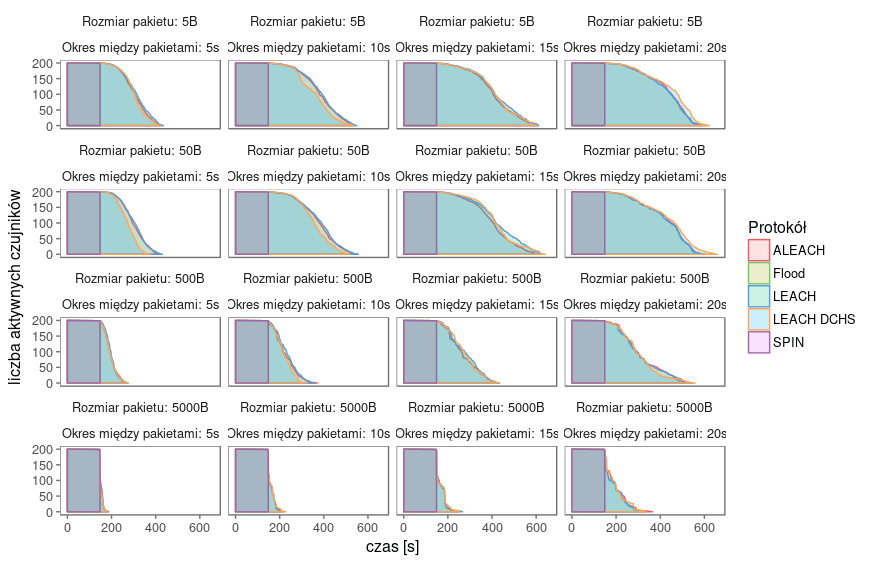
\includegraphics[width=308mm,height=229mm,page=1]{\ImgPath/charts/alive_nodes_normal_200sensors.png}}\endgraf
    \vspace{2ex}%
    \captionof{figure}{Aktywne węzły - 200 czujników, rozkład normalny}}}\kern-.5\pdfpagewidth
     \par
     \vspace*{-5cm}
\clearpage
\thispagestyle{empty}
    \vspace*{-2cm}
    \noindent\parbox{\textwidth}{%
    \noindent\rlap{\includegraphics[width=308mm,height=229mm,page=2]{\ImgPath/charts/stored_energy_normal_200sensors.png}}\endgraf
    \vspace{2ex}%
    \captionof{figure}{Energia sieci - 200 czujników, rozkład normalny}}
     \par
     \vspace*{-5cm}
\clearpage
}

\clearpage
\thispagestyle{empty}

{\pdfpagewidth=2\pdfpagewidth
    \vspace*{-2cm}
    \noindent\kern.5\pdfpagewidth\rlap{\parbox{\textwidth}{%
    \noindent\kern.25\pdfpagewidth
        \llap{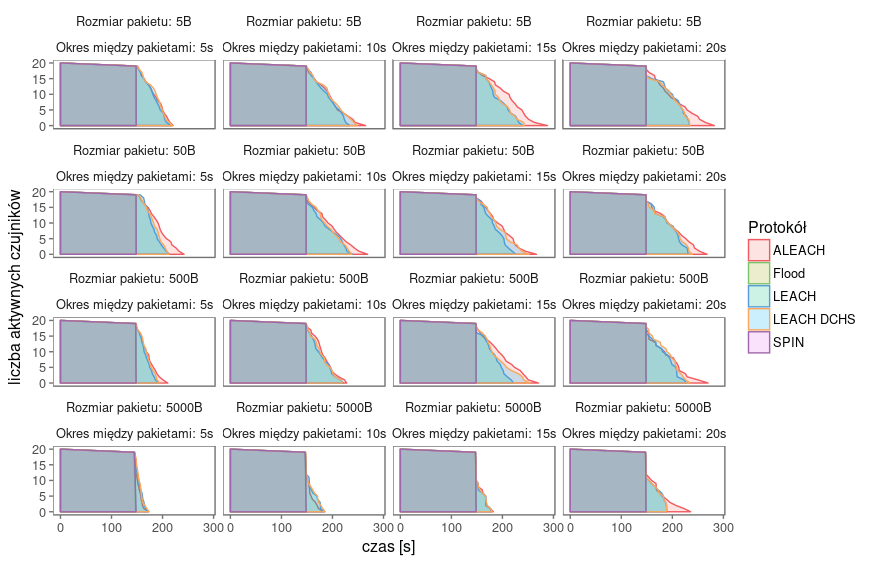
\includegraphics[width=308mm,height=229mm,page=1]{\ImgPath/charts/alive_nodes_uniform_20sensors.png}}\endgraf
    \vspace{2ex}%
    \captionof{figure}{Aktywne węzły - 20 czujników, rozkład jednorodny}}}\kern-.5\pdfpagewidth
     \par
     \vspace*{-5cm}
\clearpage
\thispagestyle{empty}
    \vspace*{-2cm}
    \noindent\parbox{\textwidth}{%
    \noindent\rlap{\includegraphics[width=308mm,height=229mm,page=2]{\ImgPath/charts/stored_energy_uniform_20sensors.png}}\endgraf
    \vspace{2ex}%
    \captionof{figure}{Energia sieci - 20 czujników, rozkład jednorodny}}
     \par
     \vspace*{-5cm}
\clearpage
}

\clearpage
\thispagestyle{empty}

{\pdfpagewidth=2\pdfpagewidth
    \vspace*{-2cm}
    \noindent\kern.5\pdfpagewidth\rlap{\parbox{\textwidth}{%
    \noindent\kern.25\pdfpagewidth
        \llap{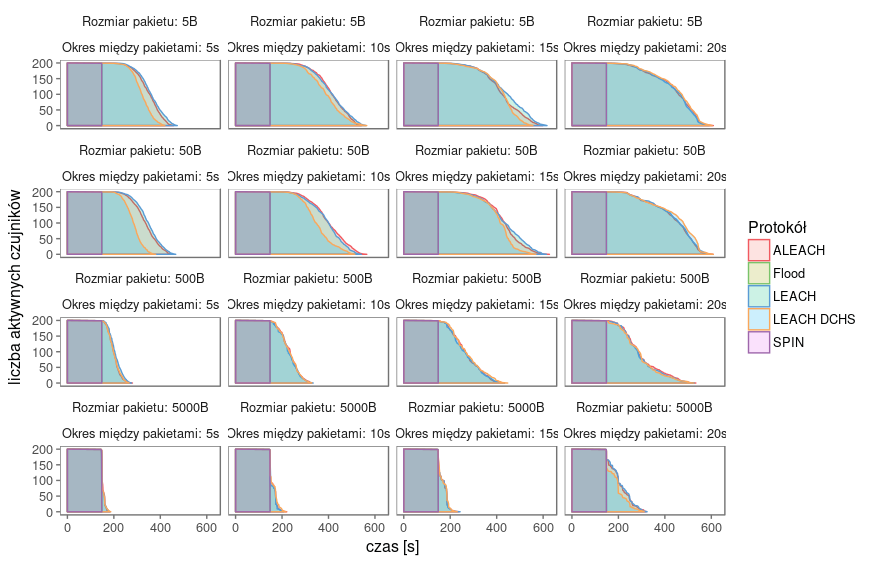
\includegraphics[width=308mm,height=229mm,page=1]{\ImgPath/charts/alive_nodes_uniform_200sensors.png}}\endgraf
    \vspace{2ex}%
    \captionof{figure}{Aktywne węzły - 200 czujników, rozkład jednorodny}}}\kern-.5\pdfpagewidth
     \par
     \vspace*{-5cm}
\clearpage
\thispagestyle{empty}
    \vspace*{-2cm}
    \noindent\parbox{\textwidth}{%
    \noindent\rlap{\includegraphics[width=308mm,height=229mm,page=2]{\ImgPath/charts/stored_energy_uniform_200sensors.png}}\endgraf
    \vspace{2ex}%
    \captionof{figure}{Energia sieci - 200 czujników, rozkład jednorodny}}
     \par
     \vspace*{-5cm}
\clearpage
}
